%%%%%%%%%%%%%%%%%%%%%%%%%%%%%%%%%%%%%%%%%%%%%%%%%%%%%%%%%%%%%%%%%%%%%%%%%%%%%%%%
%%% Problem statement
%%%%%%%%%%%%%%%%%%%%%%%%%%%%%%%%%%%%%%%%%%%%%%%%%%%%%%%%%%%%%%%%%%%%%%%%%%%%%%%%

\clearpage
\section{Problem Statement}
\label{sec:problem}

%% intro
In this section I will describe the distributed product ingestion and publishing system examined in this thesis (later: \textit{system})  and elaborate on the 
problems that I was solving. I will also describe the users of the project developed in this thesis (later: \textit{project}) and what the needs for
each of them were, as discovered by the requirements engineering work I did.

%% description of the store
%% ingestion system
%% workflows, processors, parallelism
%% description of the terms used

\subsection{The store systems}

The system being investigated in this thesis was the Microsoft Windows store.
The store sells digital \emph{products} such as games and applications.
Each product belongs to a \emph{publisher} such as an independent developer or a game company.
A product is \emph{submitted} by a publisher as a digital application package.
Before it is \emph{published} to the store catalog, it needs to be \emph{ingested},
which means the package is verified and processed through multiple steps.
After the package has been ingested and the necessary information has been collected,
it can be published, which also involves a pipeline of steps.
This involves an ingestion-publishing \emph{workflow} that consists of multiple \emph{activities} (steps).
Completion of each of these activities is logged as an \emph{event}.
The list of events for a single submission forms a \emph{trace}.
These terms will be used throughout this thesis so they shall be formally defined as follows:

% describe: workflow, trace (submission), product (bigid), publisher, event

\begin{description}[style=nextline]
\item[Product] 
Single application package being processed in the system. 

\item[Publisher] 
Independent developer or a company submitting a product into the store.

\item[Activity] 
Single step of the workflow where some part of the product is processed. 

\item[Processor] 
Part of the distributed system executing a specific activity.

\item[Workflow]
Abstract description of the whole pipeline consisting of a number of sequential and parallel activities. It contains the whole set of activities and their dependencies.

\item[Submission] 
Single execution of the workflow for a single product. Equates to a single \emph{case} in the process discovery model.

\item[Event] 
Log entry when a specific execution of an activity has finished or changed status. 

\item[Trace] 
Set of events describing current or past submission. 
A trace is tied to a specific product from a specific publisher and has information about all the activities and their execution times. 

\item[System] 
The distributed store backend system as a whole, with all the processors and other parts involved.

\item[Project] 
The new part of the system implemented in this thesis.

\label{desc:termdefinitions}
\end{description}


%% logging
The workflows are processed in the distributed system as a pipeline of steps. 
Multiple concurrent submissions are in progress at any moment of time.
Furthermore, many steps of the workflow are independent of each other.
Thus, a single submission can have multiple steps in progress at the same time.
These steps are often handled by an ''aggregator'' step which waits for 
all the parallel steps to finish before continuing the workflow process.
Figure \ref{fig:workflowexample} illustrates this.
The different steps of the workflow have different durations that differ based on
the step itself, the characteristics of the package, and the current workload of the system.
Because of these uncertainties, traces from two different submissions may differ from each other, 
since the completion order of the parallel steps is unknown.

\begin{figure}[htb]
\centering 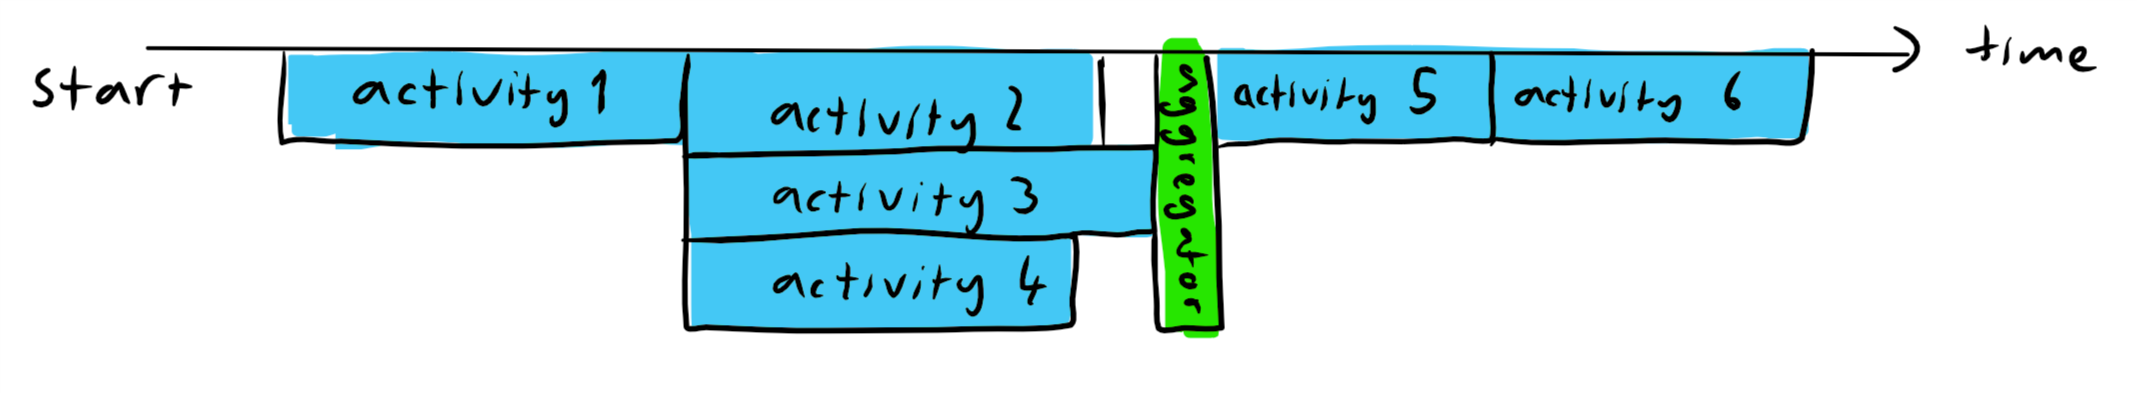
\includegraphics[width=0.9\linewidth]{gfx/figures/workflow.png}
\caption{A workflow with sequential, parallel, and aggregator steps}
\label{fig:workflowexample}
\end{figure}

When each step completes, an event is generated.
These events are collected from the different processors into a single log database.
Each step is associated with a timestamp and metadata from the event and the submissions.
The system works with a ''best effort'' delivery, which means the delivery of the events to the log database
may have undetermined delays. Furthermore, the distributed system involves multiple machines
in multiple locations. This results in variance of seconds to minutes in the clocks of the systems.
The clock variance is directly seen as noise in the timestamps of the events.

Because of the parallelism and uncertainties mentioned the overall state of the system is difficult to describe at any given time. At the time of writing the system produced on average 15~000 events per hour with peak times averaging in the 30~000 range. For the publisher of a product the system is essentially a ''black box'' where
they cannot see the internal status, only whether the workflow has been completed or if it is still in progress.

\subsection{Requirements engineering}

%% description of users
% engineers, developers, working on ingestion
% first party and third party publisher release managers
% managers, PMs
To understand the purpose of the project described in this thesis, we need to look at the users of the system
and what are their needs regarding to the project. There were five user groups relevant to the project.

\begin{description}
\item[Developers] are the software engineers working on the ingestion and publishing system.
\item[Managers] are the developer leads and program managers who coordinate the developer time and what they are working on.
\item[Publishers] are the independent developers and companies submitting the packages to the store.
\item[Release managers] are the contacts on Microsoft's side who communicate with the large publishing companies who develop the ''triple-A'' games and applications.
\item[Manual reviewers] are the people working for Microsoft that do the manual steps of the product validation when necessary. This includes for example checking for fraud or inappropriate graphics or language.
\end{description}

The needs for each user group are covered in table \ref{tab:userneeds}.
I used the ''user story'' format for documenting the needs \cite{cohn2004user}.

%% description that user needs were not fully known so they need engineering
It should be noted that the user needs were not fully understood in the beginning. The project was done in two cycles, with some necessary requirements engineering done in the beginning of both cycles. See section \ref{sec:timeline} for the project timeline. 
The user needs found at the start of the second section were related mostly on the presentation and the user interface, so they did not affect the main structure of the project significantly.

%% description of initial user needs
% which?

\begin{table}[htb]
\begin{center}
\begin{tabularx}{\linewidth}{| X |}
\hline

\textbf{As a developer I want...} \newline
- to see the current status of a submission so that I can investigate issues with a single submission or product.\newline
- to see the shape of the store workflows so that I can find issues in the dependencies.\newline
- to see statistics about the activities so that I can write reports to my superiors.\newline
- to be able to customize what I see so that I can have exactly the information I care about.\newline
- to be notified of any anomalies in the workflow so that I can investigate issues faster.\newline
- to be notified about big issues distinctively so that I can prioritize my work.
\\
\hline

\textbf{As a manager I want...} \newline
- to have statistics of the workflows so that I can report the system performance and improvements over time to my superiors.
\\
\hline

\textbf{As a publisher I want...} \newline
- to be able to know estimated times for submission completion so that I can schedule my work day.\newline
- to be able to inquire about the status of my submissions so that I can escalate any issues that arise
\\
\hline

\textbf{As a release manager I want...} \newline
- to see the detailed status of a single product or submission so that I can report it onwards. \newline
- to see the big picture status for all submissions related to a single product or publisher quickly so that I can save time. \newline
- to be notified about completion of crucial steps of the workflow or any issues so that I can schedule and prioritize my work. \newline
- to be able to customize what I see so that I do not see information about products that I do not own.
\\
\hline

\textbf{As a manual reviewer I want...} \newline
- to be notified in advance when a product is heading towards a manual review so that I can schedulemy work day.
\\
\hline

\end{tabularx}
\end{center}
\caption{Initial user needs found in January}
\label{tab:userneeds}
\end{table}

%% business requirements
%% need to integrate with an existing system
%% confidentiality, integrity
%% working with partners

There were also several business requirements from Microsoft's side for this project. They can be summarized as integration with existing systems and following confidentiality requirements. \nyi{something else?}
The project was required to integrate with the existing store backend systems. 
The event collection and storing was already handled by a system called Jury, which is an interface to browse the products in the store and see diagnostics information.
The existing system stored the events in a database and allowed the used to query the events with a SQL-like query language. The results were shown as a list of rows with the matching events and timestamps. The project was to integrate with this querying system to load the events from the database.
The events and the product metadata in the system contained confidential information. Mainly there were two terms used to classify this. First term was \textit{Medium Business Intelligence} (MBI) and the more strict was \textit{Personally Identifiable Information} (PII). In practice it meant that PII-classified information should not be visible through the interface provided by the project, and the MBI-classified information related to a product should only be shown to the publisher or the partner who owns the product. However, the developers working at Microsoft should be able to see all MBI-classified information.

%% challenges
%%  user needs not fully understood
%%  unknown parallelism
%%  unsupervised learning and adaptation
%%  both real time and statistical data are needed

There were several challenges discovered in the beginning of the project.
The system implemented in the project should be unsupervised.
This means that the system should use past data to build an understanding of the workflows, without the need for a user to supply any knowledge beforehand.
The system should adapt to any changes in the workflow automatically.
This means that the distributed workflows contain unknown parallelism that must be detected automatically.
It was also discovered that the distributed system contains noise in the timestamps which further complicate the parallelism detection.
In addition, the system should be able to provide two different kinds of information. The workflow models and statistics should be build based on a long term aggregate discovered from several days worth of data, but the system should also show the real time data for the current submissions.
These two sides of information should both be utilized in the models.
Lastly, the user needs needed some requirements engineering. This is why an iterative process was set up. Section \ref{sec:timeline} contains a detailed description of this process.

%% needs discovered at meetings?

%% conclusion, key goals
To recap, the key goals and values for the solution are the ability to dynamically adapt to changes in the workflow,
the ability for the user to customize the information they need, an decoupling the solution from the specific 
workflow steps of the store. The project needs to use \emph{unsupervised learning} to build the models, show \emph{real-time data} to the user based on the model, and use \emph{supervised learning} based on the models and the data to show predictions and send notifications.
